\documentclass[11pt]{article}
\usepackage[margin=1in]{geometry}
\usepackage{amsmath,amssymb,amsthm,graphicx,microtype,mathtools}
\usepackage[hidelinks]{hyperref}
\emergencystretch=3em

\newtheorem{theorem}{Theorem}
\newtheorem{lemma}[theorem]{Lemma}
\newcommand{\Mn}{\mathbb M_3}
\newcommand{\tr}{\operatorname{Tr}}

\title{Neither Reverse Extremal Norm Envelope Need Exist}
\author{Full counterexample packet for arXiv:1604.02812\\
\texttt{fa\_banach\_001}, lane 8, \texttt{agent\_lane\_08}}
\date{12 August 2026}

\begin{document}
\maketitle

\begin{center}
\fbox{\parbox{0.91\textwidth}{
\textbf{Status: candidate counterexample (full answer).}
On $\mathbb M_3$, an explicit norm has no greatest $L$-norm below it.
The dual norm has no least $M$-norm above it.  Thus both general existence
questions in Kian have negative answers already in dimension three.
}}
\end{center}

\section{Source question}

Kian \cite[p.~11, after Corollary 3.5]{Kian} proves the existence of the
opposite extremal envelopes and asks:
\begin{enumerate}
\item Does the class of $L$-norms below an arbitrary norm contain a greatest
element?
\item Does the class of $M$-norms above an arbitrary norm contain a least
element?
\end{enumerate}
The source answers these only in special cases.  We answer both questions in
the negative.

\begin{figure}[p]
\centering
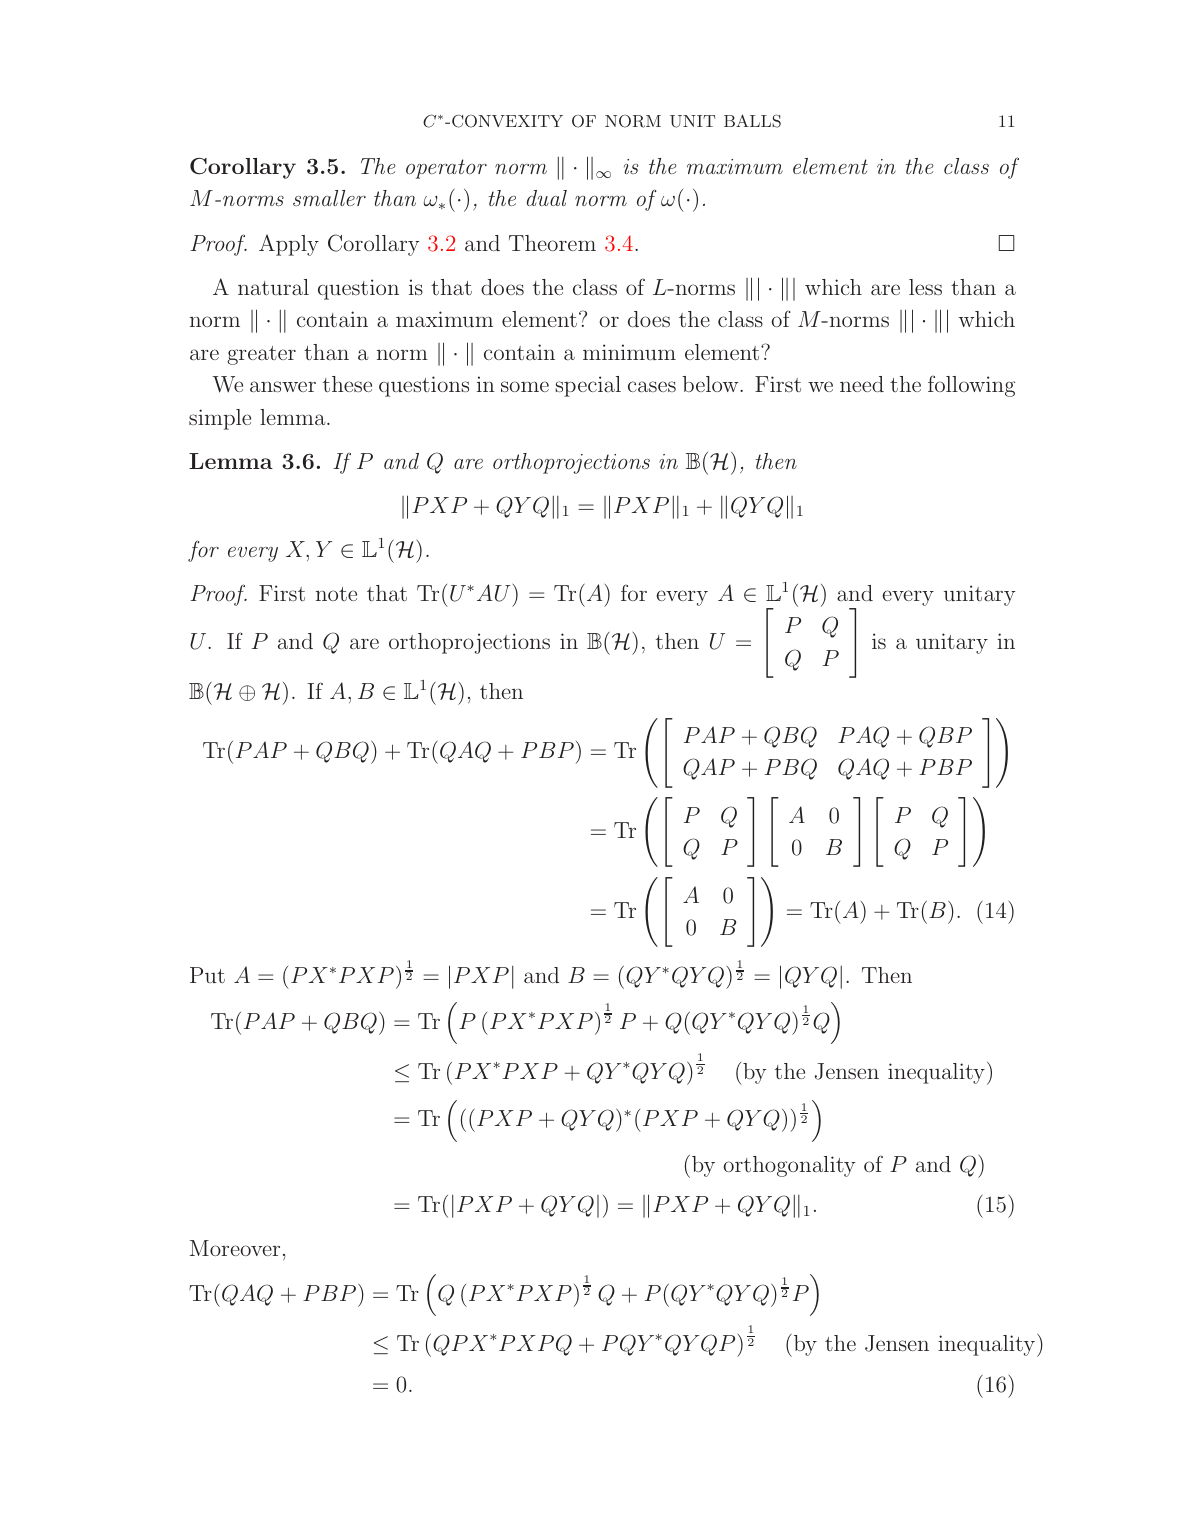
\includegraphics[width=0.96\textwidth,height=0.82\textheight,keepaspectratio]{figures/source_question_page11.png}
\caption{Source PDF page 11.  The two general existence questions appear
immediately after Corollary 3.5.}
\end{figure}
\clearpage

\section{Preliminaries}

Let $\omega$ denote the numerical-radius norm and $\omega_*$ its dual under
the trace pairing $\langle A,B\rangle=\tr(A^*B)$.  We use two elementary
facts from the source framework:
\begin{itemize}
\item the trace norm $\|\cdot\|_1$ and $\omega_*$ are $L$-norms;
\item duality reverses norm order and takes $L$-norms to $M$-norms.
\end{itemize}
For completeness, the first fact follows because the operator norm and
numerical radius are $M$-norms.  For the numerical radius this is immediate:
if $\sum C_i^*C_i=I$, then
\[
 \omega\!\left(\sum_iC_i^*A_iC_i\right)
 \leq\max_i\omega(A_i).
\]
Indeed, apply the quadratic forms to a unit vector and use
$\sum_i\|C_ix\|^2=1$.  The operator-norm statement follows by writing the
sum as a compression of the block-diagonal operator
$\operatorname{diag}(A_1,\ldots,A_k)$.

We will also use the following order-theoretic observation.

\begin{lemma}\label{lem:obstruction}
Let $a$ and $b$ be $L$-norms, and suppose $p=\max\{a,b\}$ is not an
$L$-norm.  Then there is no greatest $L$-norm below $p$.
\end{lemma}

\begin{proof}
Both $a$ and $b$ lie below $p$.  If a greatest such $L$-norm $g$ existed,
then $g\geq a,b$, hence $g\geq p$.  Since also $g\leq p$, one would have
$g=p$, contradicting the hypothesis.
\end{proof}

\section{The explicit counterexample}

Let $E=E_{11}$, $J=E_{23}$, and $X=E+J$ in $\Mn$.  Thus, relative to
$\mathbb C\oplus\mathbb C^2$,
\[
 X=1\oplus\begin{bmatrix}0&1\\0&0\end{bmatrix}.
\]
Put
\begin{equation}\label{eq:p}
 p(A)=\max\left\{\|A\|_1,\frac34\omega_*(A)\right\}.
\end{equation}
This is a norm and is the maximum of the two $L$-norms
$a=\|\cdot\|_1$ and $b=\tfrac34\omega_*$.

The relevant values are
\begin{equation}\label{eq:values}
\begin{array}{c|ccc}
 A&E&J&X\\ \hline
 \|A\|_1&1&1&2\\
 \omega_*(A)&1&2&3\\
 p(A)&1&\tfrac32&\tfrac94.
\end{array}
\end{equation}
Here is a short exact verification of the second row.  Clearly
$\omega_*(E)=1$.  Since $\omega(J)=1/2$, the test matrix $2J$ gives
$\omega_*(J)\geq2$; the reverse inequality follows from the standard bound
$\|Y\|_\infty\leq2\omega(Y)$.  Finally, the triangle inequality gives
$\omega_*(X)\leq3$, while the block-diagonal test matrix $E+2J$ has numerical
radius one and
\[
 \tr\bigl(X^*(E+2J)\bigr)=3,
\]
so equality holds.

\begin{theorem}\label{thm:counterexample}
The norm $p$ in \eqref{eq:p} has no greatest $L$-norm below it.
\end{theorem}

\begin{proof}
Let $P=E$ and $Q=I-E$.  These are orthogonal projections with
$P^*P+Q^*Q=I$, and
\[
 PXP=E,\qquad QXQ=J.
\]
The $L$-norm inequality for $p$ would require
\[
 p(PXP)+p(QXQ)\leq p(X).
\]
But \eqref{eq:values} gives
\[
 1+\frac32=\frac52>\frac94.
\]
Thus $p$ is not an $L$-norm.  Lemma~\ref{lem:obstruction}, applied to
$a=\|\cdot\|_1$ and $b=\tfrac34\omega_*$, finishes the proof.
\end{proof}

\noindent\textbf{Robustness.}
The same construction works with $\tfrac34$ replaced by every
$c\in(1/2,1)$.  Indeed, for
$p_c=\max\{\|\cdot\|_1,c\omega_*\}$ one has
\[
 p_c(E)+p_c(J)=1+2c>\max\{2,3c\}=p_c(X).
\]

\section{The dual counterexample}

Let $r=p_*$.  It can be written explicitly as the infimal convolution
\begin{equation}\label{eq:r}
 r(A)=\inf_{A=B+C}
 \left(\|B\|_\infty+\frac43\omega(C)\right).
\end{equation}
Indeed, the unit ball of the dual of a maximum is the convex hull of the two
dual unit balls.

\begin{theorem}\label{thm:dual}
There is no least $M$-norm above the norm $r$ in \eqref{eq:r}.
\end{theorem}

\begin{proof}
The two $M$-norms
\[
 q_1=\|\cdot\|_\infty=a_*,
 \qquad q_2=\frac43\omega=b_*
\]
both dominate $r=p_*$.  If a least $M$-norm $q\geq r$ existed, then
$q\leq q_1,q_2$.  Dualizing these three inequalities would give an $L$-norm
$q_*$ satisfying
\[
 a\leq q_*,\qquad b\leq q_*,\qquad q_*\leq r_*=p.
\]
Hence $q_*=\max\{a,b\}=p$, contradicting
Theorem~\ref{thm:counterexample}.
\end{proof}

\section{Scope and provenance}

Theorems~\ref{thm:counterexample} and \ref{thm:dual} settle both source
questions as universally stated.  They do not contradict the positive
special cases in the source: extremal reverse envelopes can exist for
particular reference norms, but need not exist for arbitrary ones.

A bounded literature search using the source identifier and title, the exact
``maximum $L$-norm'' and ``minimum $M$-norm'' phrases, and the relevant norm
keywords found no later paper giving this counterexample or an explicit full
resolution.  This packet is therefore presented as a new candidate
counterexample for human review.

\begingroup\raggedright
\begin{thebibliography}{9}
\bibitem{Kian}
M. Kian,
\emph{$C^*$-convexity of norm unit balls},
J. Math. Anal. Appl. 445 (2017), 1417--1427;
arXiv:1604.02812, doi:10.1016/j.jmaa.2016.04.022.
\end{thebibliography}
\endgroup

\end{document}
